\documentclass{beamer}
\usepackage[utf8]{inputenc}
\usepackage[russian]{babel}
\usepackage{amsmath,mathrsfs,mathtext}
\usepackage{graphicx, epsfig}
\usepackage{color}
\usetheme{Warsaw}%{Singapore}%{Warsaw}%{Warsaw}%{Darmstadt}
\usecolortheme{sidebartab}
\definecolor{beamer@blendedblue}{RGB}{15,120,80}
%----------------------------------------------------------------------------------------------------------
\title[\hbox to 56mm{\hfill\insertframenumber\,/\,\inserttotalframenumber}]
{Анализ тональности русскоязычных текстов\\
при помощи рекуррентных нейронных сетей\\
с механизмом внимания}
\author[И.\,С. Иванов]{\large \\Илья Сергеевич Иванов\\
{\small Научный руководитель к.ф.-м.н. Михаил Бурцев}}
\institute{\large
Московский физико-технический институт\\
Факультет Инноваций и Высоких Технологий\\
Кафедра Анализа Данных}
\date{2017}
%----------------------------------------------------------------------------------------------------------
\begin{document}
%----------------------------------------------------------------------------------------------------------
\begin{frame}
%\thispagestyle{empty}
\titlepage
\end{frame}
%-----------------------------------------------------------------------------------------------------
\begin{frame}{Цель исследования}
Исследовать новые методы анализа тональности коротких текстов на русском языке с применением рекуррентных нейронных сетей и механизма внимания.
\begin{block}{Проблемы}
	Сложная морфология русского языка.\\
	Особенности лексикона пользователей соц. сети.\\
	Малый объём данных для обучения.\\
\end{block}

\begin{block}{Предположения}
	Зависимость класса от порядка слов в тексте.\\
	Разная значимость слов в тексте при классификации.
\end{block}

\end{frame}
%-----------------------------------------------------------------------------------------------------
\begin{frame}{Литература}
	\begin{enumerate}
		\item Arkhipenko K., Kozlov I., Trofimovich J., Skorniakov K., Gomzin A., Turdakov D.. Comparison of Neural Network Architectures for Sentiment Analysis of Russian Tweets. Computational Linguistics and Intellectual Technologies. Dialog, 2016.	
		\item Zichao Yang, Diyi Yang, Chris Dyer, Xiaodong He, Alexander J. Smola, Eduard H. Hovy. Hierarchical Attention Networks for Document Classification. HLT-NAACL, 2016.
		\item Dzmitry Bahdanau, Kyunghyun Cho, and Yoshua Bengio. Neural Machine Translation by Jointly Learning to Align and Translate. ICLR, 2014.
	\end{enumerate}
\end{frame}
%----------------------------------------------------------------------------------------------------------
\begin{frame}{Постановка задачи классификации}
	\begin{block}{}
        Дано множество коротких сообщений $\mathfrak{D} = \{\mathbf{d}_j\}_{j=1}^{K}$, относящихся к компании(-ям).
	\end{block}    
    
    \begin{block}{}
        Необходимо классифицировать сообщения из $\mathfrak{D}$ на три класса:
        	\begin{enumerate}
			\item положительной тональности (положительные);
			\item отрицательной тональности (отрицательные);
			\item не имеющие тональности (нейтральные).
			\end{enumerate}
	\end{block}
	
	\begin{block}{Функционалы качества}
		Макро-усредненная F-мера
относительно классов положительных и
отрицательных сообщений.
	\end{block}
	В качестве классификатора предлагается использовать двунаправленную рекуррентную нейронную сеть с механизмом внимания.
\end{frame}
%----------------------------------------------------------------------------------------------------------
\begin{frame}{Векторное представление слов}
	\begin{itemize}
	\item Сообщение $\mathbf{d}\in\mathfrak{D}$ является последовательностью слов $\mathbf{d}=\mathbf{w}_1..\mathbf{w}_T$ из словаря $\mathfrak{W}$.\\
	\item Слово $\mathbf{w}\in\mathfrak{W}$ представляется вектором в $D$-мерном пространстве.\\
	\item Векторное представление для всех слов из словаря получается при помощи алгоритма Word2Vec, применённом на большом наборе неразмеченных данных.
	\end{itemize}
\begin{figure}[!h]
  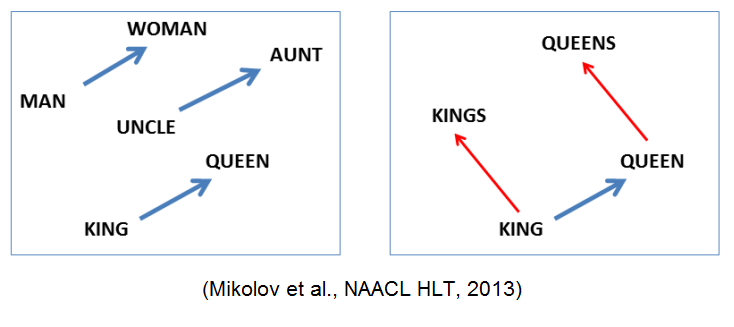
\includegraphics[width=1.0\textwidth]{images/word2vec.png}
\end{figure}
\end{frame}
%----------------------------------------------------------------------------------------------------------
\begin{frame}{Рекуррентная нейронная сеть}
	\begin{itemize}
	\item В качестве классификатора используется двунаправленная рекуррентная нейронная сеть типа GRU (Gated Recurrent Unit) с механизмом внимания.\\
	\item Функцией ошибки является перекрёстная энтропия для трёх классов.\\
	$$ J(W)=-\sum_{i=1}^{n}\sum_{k=1}^{3}y_{i}^{(k)}\log{\hat{y_{i}}^{(k)}},
	$$$$
	\hat{y_{i}}^{(k)} = \frac{\exp{s_{i}^{(k)}}}{\sum_{j=1}^{3}\exp{s_{i}^{(j)}}}
	$$
	\end{itemize}

\end{frame}
%----------------------------------------------------------------------------------------------------------
\begin{frame}{Двунаправленный GRU}
	\begin{block}{Уравнения GRU}
	\begin{align}
	z_{t}&=\sigma_{g}(W_{z}x_{t}+U_{z}h_{t-1})\\
	r_{t}&=\sigma_{g}(W_{r}x_{t}+U_{r}h_{t-1})\\
	\tilde{h}_{t}&=\tanh(Wx_{t}+U(r_{t}\circ h_{t-1}))\\
	h_{t}&=(1-z_{t})\circ \tilde{h}_{t}+z_{t}\circ h_{t-1}
	\end{align}	
% LSTM
%		f_{t}&=\sigma_{g}(W_{f}x_{t}+U_{f}h_{t-1}+b_{f})\\
%	i_{t}&=\sigma_{g}(W_{i}x_{t}+U_{i}h_{t-1}+b_{i})\\
%	o_{t}&=\sigma_{g}(W_{o}x_{t}+U_{o}h_{t-1}+b_{o})\\
%	c_{t}&=f_{t}\circ c_{t-1}+i_{t}\circ \sigma_{c}(W_{c}x_{t}%+U_{c}h_{t-1}+b_{c})\\
%	h_{t}&=o_{t}\circ \sigma_{h}(c_{t})

	\end{block}
\begin{figure}[!h]
  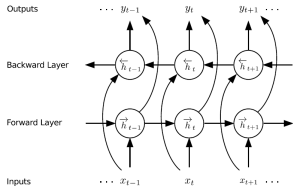
\includegraphics[width=0.5\textwidth]{images/birnn.png}
\end{figure}
\end{frame}
%----------------------------------------------------------------------------------------------------------
\begin{frame}{Механизм внимания}
	\begin{block}{Уравнения механизма внимания}
	\begin{align}
	\upsilon_{t}&=\tanh{(W_{\omega}\left[\overrightarrow{h_{t}},\overleftarrow{h_{t}}\right]+b_{\omega})}\\
	\alpha_{t}&=\frac{\exp{(\upsilon_{t}^{T}u_{\omega})}}{\sum_{j=1}^{T}\exp{(\upsilon_{j}^{T}u_{\omega})}}\\
	\upsilon&=\sum_{t=1}^{T}\alpha_{t}h_{t}
	\end{align}	
	\end{block}
\begin{figure}[!h]
  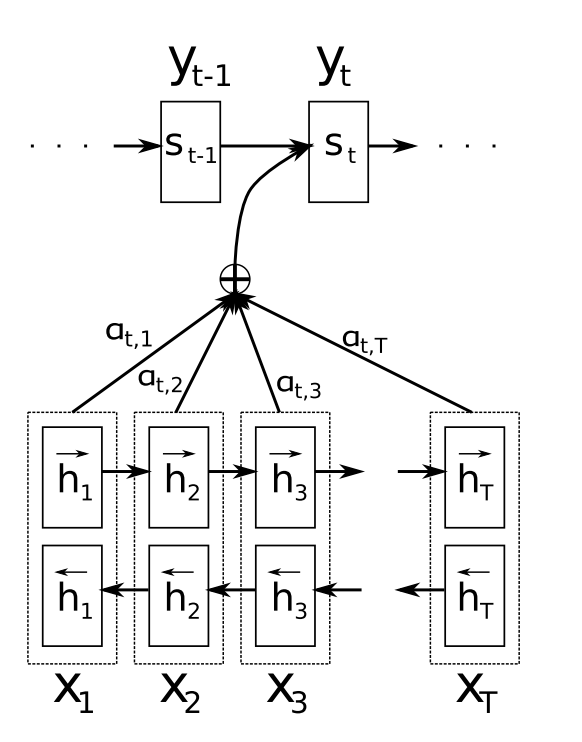
\includegraphics[width=0.25\textwidth]{images/attention.png}
\end{figure}
\end{frame}
%----------------------------------------------------------------------------------------------------------
\begin{frame}{Набор данных}
	В качестве коллекции документов $\mathfrak{D}$ используется набор сообщений пользователей соц. сети Twitter с упоминанием некоторых банков и телекоммуникационных компаний, собираемые с 2013-го года. Особенностями данной коллекции являются:
	\begin{itemize}
	\item Размер сообщения - не более 140 символов
	\item Лексикон:
		\begin{itemize}
			 \item сленг
			 \item сокращения
			 \item эмотиконы		
		\end{itemize}
	\item Спец. символы:
		\begin{itemize}
			 \item \# (хэштег)
			 \item @ (ссылка на пользователя)
		\end{itemize}
	\item Ссылки на внешние ресурсы
	\end{itemize}
\end{frame}
%-----------------------------------------------------------------------------------------------
\begin{frame}{Цели эксперимента}
	\begin{enumerate}
		\item Реализовать архитектуру двунаправленной рекуррентной сети с механизмом внимания (Python + TensorFlow)
		\item Провести подбор оптимальных гиперпараметров (GridSearch)
		\item Сравнить результаты с предложенными ранее алгоритмами.
	\end{enumerate}
\end{frame}
%----------------------------------------------------------------------------------------------------------
\begin{frame}{Вычислительный эксперимент}
В ходе эксперимента сравниваются результаты предложенного алгоритма классификации с такими алгоритмами как двунаправленная рекуррентная нейронная сеть (без механизма внимания) и метод опорных векторов. \\
\begin{block}{План эксперимента}
	\begin{enumerate}
		\item Предобработать набор текстов
		\item Обучить Word2Vec
		\item Реализовать двунаправленный GRU
		\item Реализовать механизм внимания
		\item Подобрать оптимальные параметры модели на обучающей выборке
		\item Протестировать модель на отложенной выборке
		\item Сравнить результаты с другими алгоритмами
	\end{enumerate}
\end{block}
\end{frame}
%----------------------------------------------------------------------------------------------------------
\begin{frame}{Предобработка данных}

\begin{enumerate}
	\item Токенизация (NLTK)
	\item Лемматизация (PyMorphy2)
	\item Векторизация слов (Word2Vec, обученный на русскоязычном корпусе из социальных медиа)
	\item Дополнение последовательностей нулями до максимальной длины (zero-padding)
	
\end{enumerate}
\end{frame}
%----------------------------------------------------------------------------------------------------------
\begin{frame}{Предобработка данных}

\begin{figure}[!h]
\caption{Распределение кол-ва слов в сообщении}
  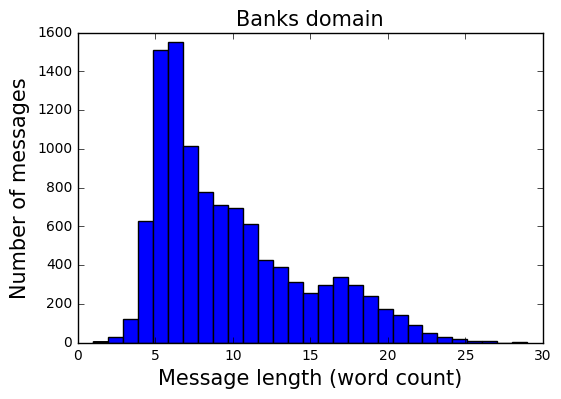
\includegraphics[width=0.5\textwidth]{images/mess_len_bank.png}
    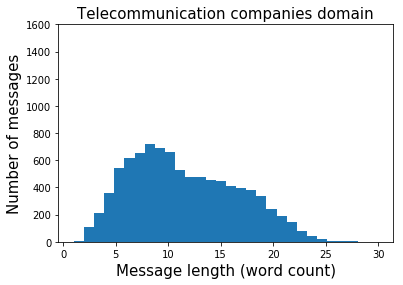
\includegraphics[width=0.5\textwidth]{images/mess_len_tkk2.png}
\end{figure}

\end{frame}
%----------------------------------------------------------------------------------------------------------
\begin{frame}{Сравнение качества полученных моделей}

\begin{table}[]
\centering
\caption{Результаты моделей на 5-фолд кросс-валидации}
\label{tab:cv}
\begin{tabular}{l|l|l|}
\cline{2-3}
                                                                                                              & \multicolumn{1}{c|}{Banks}    & \multicolumn{1}{c|}{\begin{tabular}[c]{@{}c@{}}Telecommunication\\ companies\end{tabular}} \\ \cline{2-3} 
                                                                                                              & \multicolumn{1}{c|}{F1-score} & \multicolumn{1}{c|}{F1-score}                                                              \\ \hline
\multicolumn{1}{|l|}{Bi-GRU}                                                                                  & 0.740                         & 0.625                        \\ \hline
\multicolumn{1}{|l|}{Bi-GRU + Attention}                                                                      & 0.737                         & 0.609                         \\ \hline
\multicolumn{1}{|l|}{\begin{tabular}[c]{@{}l@{}}2-layer GRU,\\ reversed sequences\\ (Arhipenko)\end{tabular}}
& 0.621                        & 0.660                                        \\ \hline
\multicolumn{1}{|l|}{Bi-GRU (Arhipenko)}                                                                      & 0.621                       & 0.652                         \\ \hline
\multicolumn{1}{|l|}{LSTM (Arhipenko)}                                                                      & 0.603                       & 0.641                         \\ \hline
\end{tabular}
\end{table}

\end{frame}
%----------------------------------------------------------------------------------------------------------
\begin{frame}{Сравнение качества полученных моделей}

\begin{table}[]
\centering
\caption{Результаты моделей на тестовой выборке}
\label{tab:test}
\begin{tabular}{l|l|l|}
\cline{2-3}
                                                                                                              & \multicolumn{1}{c|}{Banks}    & \multicolumn{1}{c|}{\begin{tabular}[c]{@{}c@{}}Telecommunication\\ companies\end{tabular}} \\ \cline{2-3} 
                                                                                                              & \multicolumn{1}{c|}{F1-score} & \multicolumn{1}{c|}{F1-score}                                                              \\ \hline
\multicolumn{1}{|l|}{Bi-GRU}                                                                                  & 0.48                          & 0.52                                                                                       \\ \hline
\multicolumn{1}{|l|}{Bi-GRU + Attention}                                                                      & 0.51                          & 0.49                                                                                       \\ \hline
\multicolumn{1}{|l|}{\begin{tabular}[c]{@{}l@{}}2-layer GRU,\\ reversed sequences\\ (Arhipenko)\end{tabular}} & 0.55                          & 0.56                                                                                       \\ \hline
\multicolumn{1}{|l|}{CNN (Arhipenko)}                                                                      & 0.48                          & 0.47                                                                                       \\ \hline
\multicolumn{1}{|l|}{SVM baseline}                                                                      & 0.46                          & 0.46                                                                                       \\ \hline
\multicolumn{1}{|l|}{Majority baseline}                                                                      & 0.31                          & 0.19                                                                                       \\ \hline
\end{tabular}
\end{table}

\end{frame}
%----------------------------------------------------------------------------------------------------------
\begin{frame}{Заключение}

	\begin{itemize}
		\item Реализован алгоритм двунаправленной рекуррентной нейронной сети с механизмом внимания для классификации тональности коротких русскоязычных текстов. Код отлажен и выложен в открытый доступ
		\item Проведён поиск оптимальных гиперпараметров алгоритма
		\item Проведено сравнение результатов с предложенными ранее алгоритмами
		\item Подготовлен отчет по результатам работы
	\end{itemize}

	\begin{block}{Дальнейшее исследование}
		Исследование применимости данной модели в качестве модуля для нейронной сети, генерирующей сообщения с заданной тональностью.
	\end{block}
\end{frame}
%----------------------------------------------------------------------------------------------------------
\end{document} 